%\documentclass{acm_proc_article-sp}
%\documentclass[10pt]{sig-alternate-10pt}
\documentclass{sig-alternate-11pt}
\usepackage{amsmath}
\usepackage{amssymb}
\usepackage{listings}
\usepackage{courier}
\usepackage{multirow}

% Include PDF graphics, configure our images directory, and specify image types.
\usepackage{graphicx}
\usepackage{epsfig}
\graphicspath{{./images/}}
%\DeclareGraphicsExtensions{.pdf,.jpeg,.png,.jpg}
\DeclareGraphicsExtensions{.eps}

% Style listings
\lstset{%rulesepcolor=\color{Gray},
        frame=single,                        	% Shadow box frame around code
        basicstyle=\scriptsize\ttfamily,        % Use small true type font
        showstringspaces=false,                 % Don't put marks in string spaces
        morecomment=[l][\color{Blue}]{...},     % Line continuation (...) like blue comment
}

\begin{document}

\title{A Domain Specific Language for Usage Management}

\numberofauthors{1}

\author{
\alignauthor
Christopher C. Lamb, Pramod A. Jamkhedkar, Mathew P. Bohnsack, Viswanath Nandina, Gregory L. Heileman \\
       \affaddr{University of New Mexico}\\
       \affaddr{Department of Electrical and Computer Engineering}\\
       \affaddr{Albuquerque, NM 87131-0001}\\
       \email{\{cclamb, pramod54, mbohnsack, vishu, heileman\}@ece.unm.edu}
}

\conferenceinfo{DRM'11,} {October 21, 2011, Chicago, Illinois, USA.} 
\CopyrightYear{2011} 
\crdata{978-1-4503-1005-5/11/10} 
\clubpenalty=10000 
\widowpenalty = 10000

\maketitle

\begin{abstract}
In this paper we describe the development of a domain specific language (DSL) for expressing usage management policies and associating those policies with managed artifacts.  We begin by framing a model for the language, including generalized use cases, a domain model, a general supported life-cycle, and specific extension requirements.  We then develop the language from that model, demonstrating key syntactic elements and highlighting the technology behind the language while tracing features back to the initial model.  We then demonstrate how the DSL supports common usage management and DRM-centric environments, including creative commons, the extensible rights markup language (XrML), and the open digital rights language (ODRL).
\end{abstract}

\category{D.3.0}{Software}{Programming Languages}[General]
\terms{Design, Languages, Security}
\keywords{Access Control, Interoperability, DRM, Usage Management}

\section{Introduction}
For the purposes of this paper, we current define usage management as the management of the usage of resources (and data) across and within computing environments.  More than access control or digital rights management, usage management concerns itself with fine-grained control of all aspects of how a given digital resource is used.  As digital environments become more open over time, the need for usage management for resources that span utility computational environments (e.g. cloud provider systems) will become increasingly important.

With the advent and widespread use of cloud computing, those responsible for a given usage managed resource are almost never those responsible for the computing systems, except at edge devices like mobile phones or other small profile computing devices.  Resources are regularly moved across national boundaries and regional areas without either the content owner's or creator's knowledge.  Furthermore, this kind of transfer is generally according to pre-established algorithms or data routing protocols over which users of all stripes have no control.  Managing these kinds of issues requires new usage management capabilities that can run on platforms ranging from small, hand-held devices to nodes in large data centers.

Historically research in this area has been focused on developing more expressive policy languages via either different type of mathematical logics or formalisms with greater reasoning capabilities~\cite{ArHu:07,BaMi:06,ChCoEtHaJoLa:03,HaWe:04,HaWe:08,PuWe:02,XiBjFu:08}.  These approaches however fail to address interoperability challenges posed by new commercially available distributed computing environments.Interoperability efforts have resorted to translation mechanisms, where the policy is translated in its entirety to a different language~\cite{HeJa:05,PoPrDe:04,ScTaWo:04}; it has been shown recently however that such techniques are infeasible and hard to perform for most policy languages~\cite{KoLaMaMi:04, SaShUe:04}. Other approaches have led to complex policy specification languages that have tried to establish themselves as the universal standard~\cite{OMADRM,ODRL-req,Wa:04,XrML-spec}.  This unfortunately tends to stifle both innovation and flexibility~\cite{HeJa:05,JaHe:04,JaHe:08,JaHeMa:06}.

To address these issues, we first applied the principles of system design to develop a framework for usage management in open, distributed environments that supports interoperability. These principles have been used by researchers in large network design create a balance between interoperability and open, flexible architectures~\cite{Al:04,BlCl:01,ClWrSoBr:02}, allowing for computing scale and power without sacrificing innovation. Initially we standardized certain features of the framework operational semantics, and left free of standards features that necessitate choice and innovation.

We have implemented this framework, including a usage management calculus providing a platform usage management, within a Domain Specific Language (DSL) and associated evaluation environment. The DSL and its environment implements our previously defined framework, separating various roles needed for distributed policy creation and management, provides the capability to develop executable licenses, and is extensible from both a policy and constraint definition perspective.

In this paper, we will first review the problems in usage management in more detail.  Then, in Section \ref{sec:model} we will first review the model we developed to guide the DSL's syntactic and semantic development.  Then, in the next section, we will cover the language itself, how it was developed, and its supporting evaluation environment.  We will then close the paper with three specific implemenation examples showing how the language and its runtime support usage management scenarios from three different environments --- creative commons (CC), the extensible rights markup language (XRML), and the open digital rights language(ODRL).

\section{Motivation}\label{sec:motivation}
Here, we lay out the historical development of usage management and define its scope and constituent elements, tracing its origins to access control and digital rights management. Following this, we explain the challenges that result from the evolving nature in which information is being used across systems. 

\subsection{Access Control}
Access control mechanisms are systems that manage controlled access to resources. The central idea behind access control is that access to a resource is granted depending upon subject attributes, object attributes, and system attributes. The central component of any access control system, is an access control language (ACL) that is used to express rules for granting access to different resources in the system.

Access control policies can be categorized into two types, namely, discretionary access control (DAC) and mandatory access control (MAC)~\cite{HuFeKu:06}. DAC policies are  the policies that are specified by the owner of the resource, based on the users' attributes. On the other hand MAC policies are made by a central authority and apply to the whole system.  A number of access control models have been developed that allow different types of access control in these two modes. The most successful ones being the role-based access control model (RBAC), and the Bell and LaPadula model~\cite{BL:73,BL:76}. The focus of access control models is to capture the different types of relationships between and among a set of resources and a set of users, and express access rules based on those relationships. 

Access control mechanisms are generally tightly coupled with the system in which they are deployed. Situations where users identities are not known apriori requires system agnostic authentication mechanism like public key infrastructure. 

\subsection{Digital Rights Management}
Digital rights management (DRM) consists of mechanisms that manage controlled usage of digital resources. The central idea behind DRM is that usage rules for a given resource are specified for a particular user or group of users, and the use of that resource is then managed for a finite period of time.  The usage rules generally include a set of permissions and obligations, along with rules specifying how the permissions may be exercised over a period of time and under what circumstances. DRM also includes mechanisms such as trusted computing that ensure the enforcement of rights on various user systems~\cite{SaSt:04}. The most well known, but unsuccessful, approaches to address this problem are IBM's Cryptolopes and Microsoft's Palladium technologies~\cite{CaJuPoLe:02,IBM:02,KoLoKa:97}.  Given the problem of enforcing DRM, researchers have proposed incentive based, game-theoretic approaches for DRM~\cite{HeJaKhHr:07,ZhPeMaYaHa:09}. The central component of DRM systems is a rights expression language (REL) that is used to express usage rules (or rights) in the form of a license that is generated by a resource owner for a user or a group of users that will use a resource.  

Some of the earliest attempts at DRM date back to 1980's, and involve the development a formal language for legal discourse~\cite{Bo:88,McG:88,McC:89}. At present, creative commons, along with two XML-based RELs, namely, XrML and ODRL, are most commonly used~\cite{XrML:02,Ia:00}. Both XrML and ODRL have formed alliances with major players in the industry and standards bodies.  Semantics of these XML-based languages are informal. A number of approaches using various types of formalisms and approaches have been used to develop formal RELs. Gunter et al.~\cite{GuWeWr:01} and Pucella et al.~\cite{PuWe:02} have used trace-based semantics to develop formal RELs. Other formalisms such as first-order logic and CafeOBJ have been used to develop RELs~\cite{ArHu:07,ChCoEtHaJoLa:03,XiBjFu:08}. Many researchers have attempted to provide formal semantics for existing XML based RELs~\cite{HaWe:04,PuWe:06,HaWe:08}. It is however the general agreement that popular XML-based RELs are difficult to formalize in their entirety~\cite{HaWe:04,HaWe:08,JaHeMa:06}. ,

More recently, researchers have tried to expand the the concept of DRM to propose concepts including usage rights management and usage control. The idea of usage rights management is developing along the lines of making users aware of how a resource is supposed to be used~\cite{HuPaGr:09}. A more formal framework, $UCON_{ABC}$ encompassing usage rules and access control has been proposed by Park et al.~\cite{PaSa:04}.

\begin{figure}[t]
 \centerline{\includegraphics[width=3.5in]{usage_management}}
 \caption{The primary elements in a usage management system.} \label{UM}
\end{figure}

\subsection{Scope of Usage Management}
Before we discuss the scope and components of usage management, it is important to note the difference between ACLs and RELs. Even though the goals of these two types of languages overlap, the focus of research in ACLs and RELs is significantly different.  ACLs focus on defining access rules in terms of relationships between sets of resources and sets of users. In DRM systems, once a user obtains a license for a resource, access to that resource is implicit, and what matters is how that resource is used from that point onwards. Therefore, RELs  focus on defining different types of usage rules for a given user (or group of users) over a given resource (or group of resources). 

We introduce the concept of usage management that is built upon the term {\em usage control} introduced by Park et al.~\cite{PaSa:04}. The usage control model, called  $UCON_{ABC}$, is based on {\em Authorizations, oBligations and Conditions}~\cite{PaSa:04}. $UCON_{ABC}$ combines access control and  permissions and obligations in a single model. 

We now describe the components of usage management as shown in Figure~\ref{UM}, and how they relate to each other. Usage management is a combination of usage control and DRM.  Usage control is a combination of access control and usage rules. Digital rights management includes content management, license management, specification of usage rules and a simplified subset of access control.  Content and license management include processes that manage how content and license are bundled, encrypted and distributed or managed across multiple clients. These processes include encryption mechanisms, trust management, trusted computing platforms and other such management techniques. Many RELs, including XrML and ODRL, have tried to incorporate these functionalities. 

Next, we discuss challenges in implementing usage management systems, and the need for an actionable framework for addressing the challenges. 

\subsection{Challenges in Usage Management}
Unlike classical access control systems, information is increasingly used across highly networked, distributed computing environments that are not a part of a single centrally managed system.  In addition, digital information is increasingly used in innovative ways in which it is transformed, processed or merged with other information while being used across computing environments.  This necessitates usage management policies to be tightly coupled with the resource it controls rather than systems upon which that resource may reside. The policy is then interpreted and enforced as the resource moves across different computing environments. 

A logical approach to this problem is to build an interpreter for the policy language that runs on the computing environment (or the client), and enforces the policy on the client. This approach has been very successful for access control systems, because access control policies are tightly coupled with computing environments whose nature is known apriori.  However, in usage management scenarios where resources move across environments that are not known apriori, such an approach is infeasible. To address such a situation, each of the computing environments must incorporate an interpreter and enforcement mechanism that is custom built for different policy languages. 

One of the solutions to this situation is the use of a standard usage policy language for all types of information management ecosystems. Rights expression languages such as XrML and ODRL have been adopted separately as standards by different industry alliances. The semantics of these XML-based languages are informal, and researches have demonstrated the difficulty involved in providing formal semantics for these languages~\cite{HaWe:08}. 

At the same time, numerous formal logic-based rights expression languages have been developed by academicians. These languages use different types of mathematical logics to express and reason over various types of usage semantics. Both XrML and ODRL have developed and continue to develop independent of these formal languages, and have not been able to incorporate their expression and reasoning power.  Hence, unlike formal access control models, these formal languages continue to remain outside the remit of industry alliances. 
 
As a result, none of these languages are likely to become the {\em defacto} industry standard in the future.  Different information ecosystems will continue to use different policy languages according to the policy expression requirements. Such a fragmented use of policy languages will remain the biggest obstacle to achieving usage management along with unhindered flow of information across highly distributed computing environments. This implied existence of multiple policy languages in such scenarios leads to two clear problems --- difficulty supporting multiple languages and lack of interoperability.

\noindent{\bf Multiple Language Support}.
If a given computing platform intends to be a part of multiple information ecosystems, it must support the policy languages used by each of these ecosystems. This means that policy language interpreters for each of these policy languages need to be custom built for that particular computing platform. Furthermore, any advances or changes that are made in these policy languages will require corresponding updates in the interpreters used in all the computing platform.  This implies that infrastructure as a service providers like Amazon or Rackspace would need to coordinate the installation of support for the same policy languages in virtual machine instances or lock potential clients out of their systems.

\noindent{\bf Interoperability}.
The second disadvantage is that even though a given computing platform may support multiple information ecosystems, each of these information ecosystems still operate in complete isolation from one another.  Since different ecosystems use different policy languages, licenses expressed within one ecosystem cannot be interpreted in another ecosystem. This prevents resources from moving freely across different ecosystems. 

A number of recent papers have provided interesting solutions addressing interoperability at this level~\cite{marlin,coral,KoLaMaMi:04,SaShUe:04,ScTaWo:04}. The most common approach to interoperability has been translation mechanisms that translate a policy from one language to another language.  It is, however,  extremely difficult to effect this translation~\cite{HeJa:05}. The Coral and Marlin initiatives have provided architectural solutions to DRM interoperability~\cite{marlin,coral}. In the Coral approach, different licenses for different DRM systems are generated from a common token in accordance with a common ecosystem~\cite{coral}. In the Marlin approach, licenses are expressed programmatically in the form of control objects to prevent dependence on any one particular REL~\cite{marlin}. Both Coral and Marlin architectures focus on the management of licenses across systems.\\ 

The DSL we describe, in tandem with its runtime, embodies an interoperable framework for usage management, unlike Coral and Marlin architectures, that implements a formal calculus to reason about the relationship between a license, a computing environment, and interoperability between them. It incorporates concepts such as programmable licenses and common ecosystems used by Coral and Marlin architectures respectively. The usage management framework design is based on the principles of {\em design for choice}, eloquently described by Clarke et al. with reference to ``tussles'' in cyberspace~\cite{ClWrSoBr:02}. They explain the importance of identify the locations in the architecture where standards need to be introduced to enable interoperability, and locations where they should {\em not} be applied to enable innovation and differentiation.  This DSL supports that kind of differentiation by supporting for pluggable evaluators that allow users to extend the basic language syntax, semantics, and runtime arbitrarily.
\section{Language Model}\label{sec:model}
In developing this DSL, we needed to have a clear understanding of the specific domain, and develop and appropriate domain model to guide our efforts.  Admittedly, there exist many possible models that can describe this area of policy and policy management, and the model that we chose to initially use is purposefully simple to help ease development and implementation efforts.  We did however provide arbitrary language-level extensibility to support future extension into more demanding policy implementation areas.

We developed this model to help us understand how policy-centric DSLs would be used, to visualize how the various elements are inter-related, and to clarify important areas upon which to focus effort.  Through this model, we were able to conceptualize the initial language structure and generate performance hierarchies, as well as to tailor expected DSL use.

\subsection{Expected Use}
In order to develop the appropriate DSL giving users the power and expressivity they need to easily express usage management concepts, we begin by developing a model describing how we expect it to be used, and by whom, identifying key functional and non-functional characteristics.  We use roles codified as actors to identify the primary user base, and link those roles to specific use cases we expect to be common in day to day DSL use.  We also identify common inputs and outputs from expected activities, and show how those input and output elements are related.  We finally specify the essential core structure of the DSL, as well as extension points and default implementations of those points.

In general day to day use, we expect that certain activities will be much more common that others.  For example, each \textit{policy} requires a \textit{context} in order to both be developed and to run.  That \textit{context} describes the actors using an artifact protected by a policy, the artifact itself, and the environment in which the artifact is both expected to be used (during policy design) and is being used (at evaluation).  That said, the expectation is that the number of policies is much greater than the number of contexts associated with those policies.

Likewise, we expect that the number of times a policy is evaluated is much greater than the number of times that policy is designed and created.  Policies should be read, evaluated, or combined with other policies frequently.  This gives us a magnitude ordering for these activities, where the number of supported contexts is much less than the number of created policies, which is in turn much less than the number of times that policy is evaluated or otherwise used.

This has specific implications on both the DSL syntax and performance profile.  For example, as it is much more common for policies to be evaluated than contexts to be created, our efforts and tuning the system and increasing performance are best focused on policy evaluation rather than contextual activities.  In a similar vein, the language itself should be as simple to comprehend as possible for policies at the expense of contextual elements if necessary.

\begin{figure}[!t]
\centering
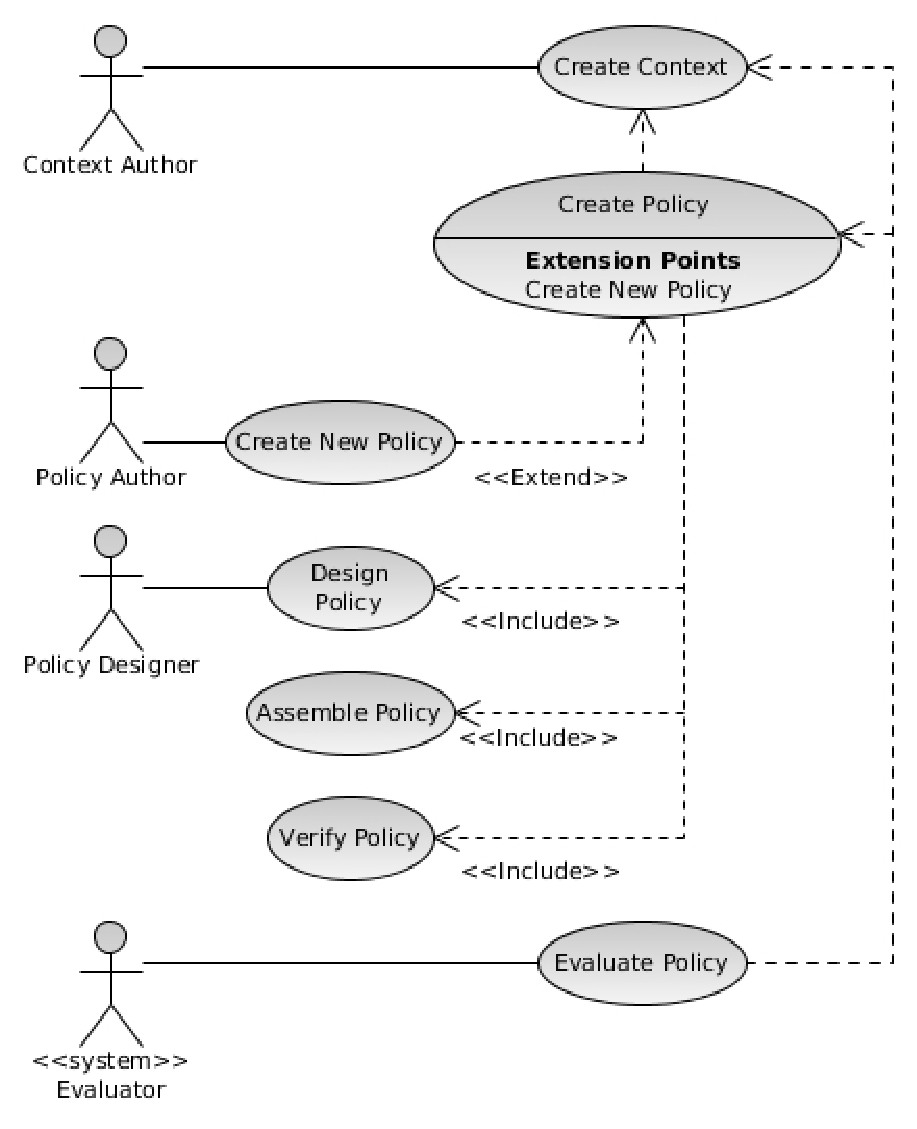
\includegraphics[width=3in]{use-cases}
\caption{General DSL Use Cases}
\label{fig:model:use-cases}
\end{figure}

Figure \ref{fig:model:use-cases} shows the primary system actors we have identified as well as the use cases with which they will be involved.  Actors include:
\begin{itemize}
\item \textit{Context Author}.  The context author is responsible for defining the context in which a policy will be applied to a given resource.  The context itself defines the environment in which the policy executes, the resource to which the policy is applied, and the subject that attempts to use the resource.
\item \textit{Policy Author}.  The policy author creates a policy to control the use of a subject defined in the policy context.
\item \textit{Combinator}. A system element, generally.  A combinator in this context combines two or more policies into a single composite policy.
\item \textit{Content Owner}.  The owner of a protected resource.
\item \textit{Evaluator}. Another system element, an evaluator evaluates a given policy with a specific context.
\end{itemize}

When a context author creates a context, that author compiles the elements of that context for use both at policy creation and policy execution.  When the policy is initially created, the resource is the only defined element.  Generally both the subject, representing the eventual user, and the environment, containing information describing the evaluation environment, are only defined at the classifier level.  That is to say, they both are defined, but individual properties have yet to be assigned.

Creating a policy is an activity undertaken by either a policy author or a combinator.  This step requires a \textit{declared} (but not \textit{defined}) context.  This is also undertaken in tandem with some kind of policy specification that describes roughly what the policy should manage and how it should be managed.  In the ontology we have defined, this is the step at which the author defines the various constraints, activities, restricted activities, and obligations.  Creating a new policy is precisely what it describes - creating a brand new policy applied to a context.  Creating a composite policy, on the other hand, involves creating a new derivative policy from two or more previously existing policies.

The included cases define policy, assemble policy, and verify policy are common development steps through which the policy is essentially designed, developed, and then tested against a context.

Once a policy has been created, the content owner can then associate that policy with a resource, essentially instantiating the resource in the associated context.

Finally, a policy is evaluated by an evaluator, a system actor, after creation and association with a resource.  At this point, the context has a fully instantiated context, with defined resource, subject, and environmental elements.

Now we have a general understanding of the expected use of a given policy, and have defined the expected roles.  With this in place, we begin to look at the elements the DSL should have to allow it to express the use cases we expect we need to support as the next step in refining our understanding of what this DSL should look like.

\subsection{Domain Ontology}
Our domain ontology will be the foundation of our DSL.  It will allow us to begin to understand the various language elements and how they are related, leading us to an eventual syntax to represent these classifiers and relationships.  Not understanding this structure well, or developing a structure that does not support our defined use cases will lead us to develop a DSL that inadequately supports our expected use.

Based on our use cases, we know the ontology contains a \textit{context}, some kind of policy-specific sub-ontology, and a logic engine that can act over that sub-ontology.  Based on our current understanding of our needs, the sub-ontology contains \textit{obligations} and \textit{constraints} applied to \textit{activities}.  We use simple propositional logic to reason over the policy elements.

This understanding leads us to the Ontology view in Figure \ref{fig:model:ontology}.  Of special note, the specific policy sub-ontology is represented as a realization of a more general \textit{policy ontology} type.  Likewise, the logic used to reason over the policy elements is propositional logic.  Both of these can change within this model to allow for inclusion of more complex policy systems and powerful reasoning capabilities.

\begin{figure}[!t]
\centering
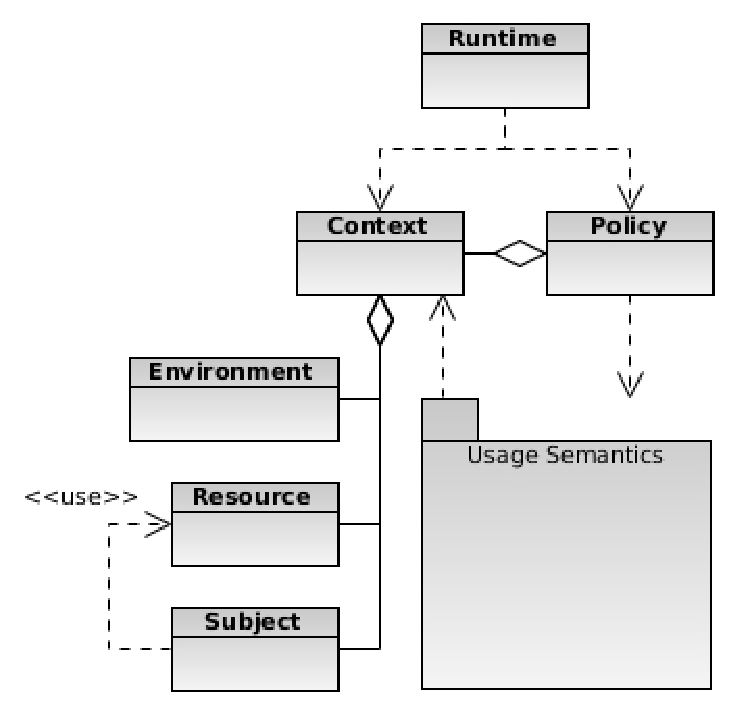
\includegraphics[width=3in]{ontology}
\caption{Basic Language Ontology}
\label{fig:model:ontology}
\end{figure}

Primary elements within this ontology are:
\begin{itemize}
\item \textit{Runtime}.  This is the system that manages use of a given \textit{resource} by a \textit{subject} in accordance with a \textit{policy}.  It is responsible for providing and managing context elements, controlling policies and licenses, and handling requests from subjects.  Realizations of this system must be cross platform to support distributed use as well.
\item \textit{Context}.  The context describes the operating environment of the policy.  This information must be available at runtime, and parts of it must be understood when the policy is initially designed.  In order to effectively control use of a given artifact, the parameters that artifact can be used under must be understood when the policy is created and must be read when that policy is evaluated.
\begin{itemize}
\item \textit{Environment}.  The environment in which a given policy is evaluated.  This must be understood in order to constrain the conditions where a policy will allow or disallow artifact access.  This is essentially an associative array, where the keys are specific expected properties of a given environment.
\item \textit{Resource}.  A resource is the artifact over which the policy controls use.  This can be any type of artifact whatsoever, ranging from documents to media files to streaming data.  A resource may also have arbitrary properties like an associated URI, a canonical name, a MIME type, or creation metadata.
\item \textit{Subject}.  Subjects use a given resource.  Acceptable use is described by the policy.
\end{itemize}
\item \textit{Policy}.  A policy describes the conditions of use for a given resource.  In our example, this includes information on acceptable contexts and subjects, as well as obligations and constraints.  Policies can be configured in this DSL to use arbitrary evaluators.  This allows users to implement specific policy semantics tailored to their domain if needed, though they are free to use packaged syntax evaluators if those evaluators fit their needs. 
\item \textit{Policy Ontology (\textsc{Abstract})}.  As policies can implement arbitrary semantics, they can be based on an ontology tailored to the needs for the particular policy system.  For example, this DSL currently implements obligations and constraints restricting defined activities.  Other domains may need to use more descriptive semantics, perhaps addressing causality or ordering.
\item \textit{Simple Ontology}.  The ontology currently used for policy development and packaged with the DSL.
\begin{itemize}
\item \textit{Obligation}.  An obligation describes something that must have occurred or must occur in the future for a restricted activity to be performed.  For example, a media stream may wish to obligate users to purchase access to that stream on the third access. 
\item \textit{Constraint}.  A constraint generally constrains the a restricted activity.  This could be as simple as limiting use to a single identifiable subject or as complex as limiting use based on time and date, user identity, and geographic location.
\item \textit{Activity}.  A general activity is something a subject would wish to do in association with an artifact.  It describes how a \textit{subject} would use a \textit{resource} in an unrestricted way.
\item \textit{Restricted Activity}.  When an activity is embellished with constraints or obligation, it becomes restricted.
\end{itemize}
\item \textit{Policy Logic (\textsc{Abstract})}.  As the general policy ontology can be changed to reflect different policy conditions, so to can the logic used to evaluate that policy change.  Recognizing this logic as a first order system element helps facilitate that substitution.
\item \textit{Propositional Logic}.  The logic currently used for policy evaluation.
\item \textit{License}.  An instance of a defined policy that would be applied to a resource.
\end{itemize}

Now we have rigorously defined the domain elements our DSL will address.  Keep in mind, this domain model allows us to dynamically replace ontology elements in that all \textit{policy ontology} and \textit{policy logic} elements can be replaced on per-policy basis.  This would allow us to create multiple policies described using disparate ontologies and related evaluation logics if needed to more fully describe restrictions in a specific evaluation domain.

We have also separated the definition of \textit{activities} from \textit{restricted activities}.  This separation of concerns allows policy developers to define a single activity which can then be reused across a large number of restricted activities based on specific varying constraints.  For example, if I have a write activity, I can constrain that activity in slightly different ways to create a relatively large number of related restricted activities.  I could restrict write by geographic area, by subject identification, by date and time, or by having contributed to some political cause, creating four restricted activities from the same base activity.

The base domain model however, based on contextual elements, policies, and licenses does not change.  This stability allows for ease of runtime integration as it hides any policy evaluation-specific changes.  As long as a given logic and policy ontology is delivered with a given policy, the policy evaluation runtime will be able to evaluate that policy against resources and subjects in a given environment.

\subsection{Envisioned Lifecycle}

\begin{figure}[!t]
\centering
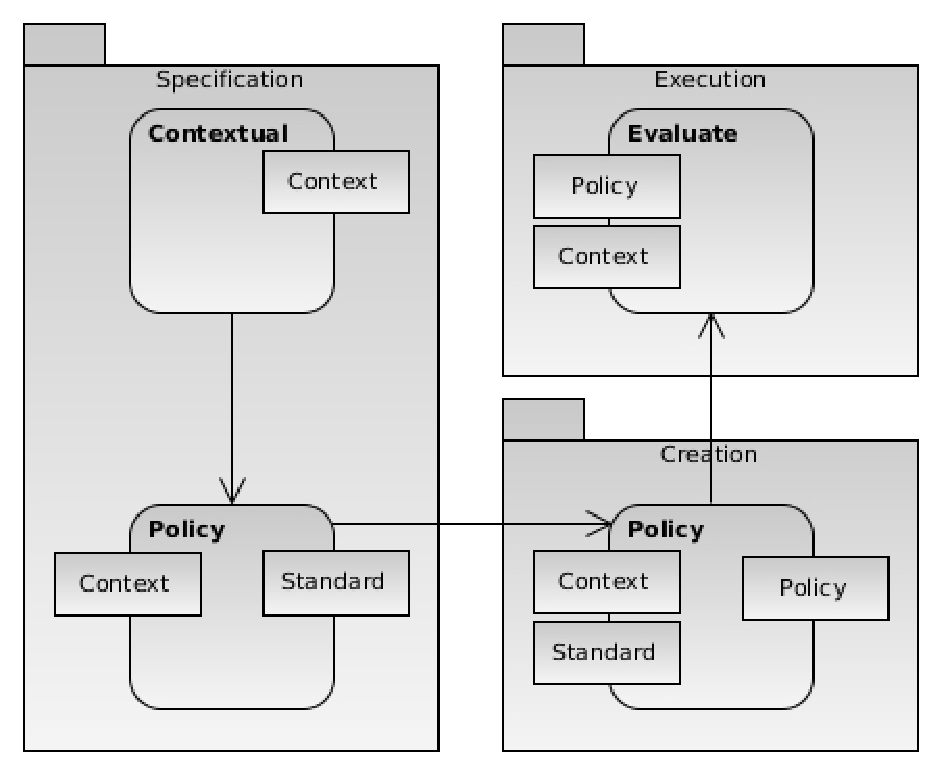
\includegraphics[width=3in]{lifecycle}
\caption{Policy Development Lifecycle}
\label{fig:model:lifecycle}
\end{figure}

\subsection{Language Components}

\begin{figure}[!t]
\centering
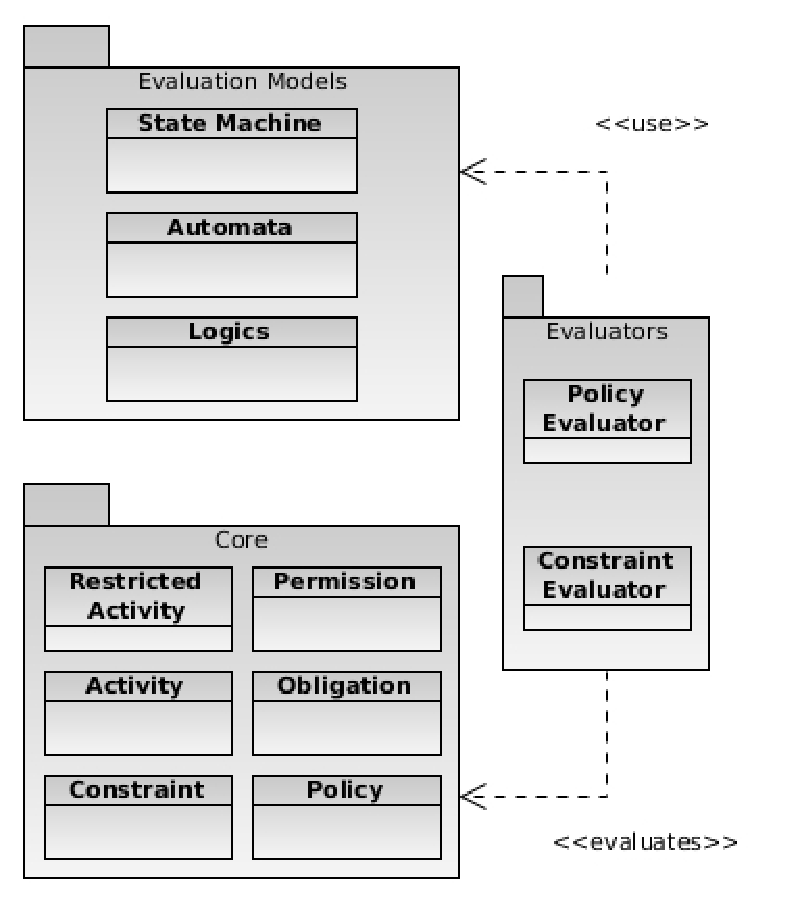
\includegraphics[width=3in]{language-components}
\caption{Language Elements}
\label{fig:model:language-components}
\end{figure}

\section{Language}\label{sec:language}
This section describes the domain specific language built upon the language model described in Section~\ref{sec:model}. First the deployment of the language is provided that explains how the DSL is operates and is used in usage management systems. This is followed by a detailed example of the syntax and semantics, and major components of the language. Finally, we demonstrate how the language can be extended to include different types of evaluators deploying different types of logics. 

\begin{figure}[!t]
\centering
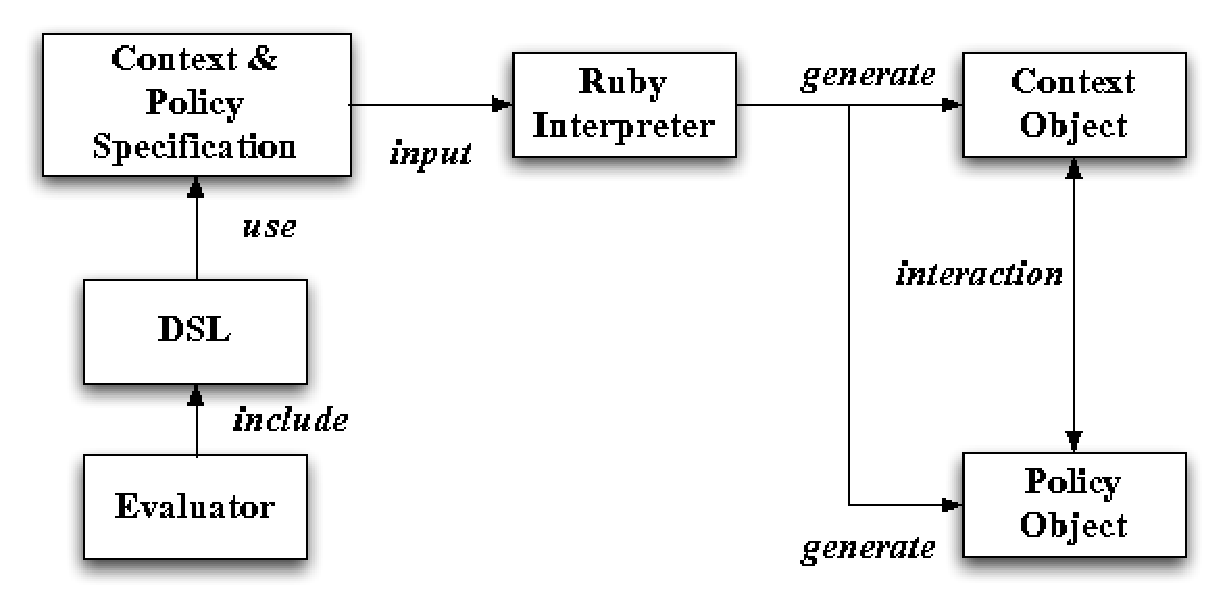
\includegraphics[width=3.5in]{DSL-usage}
\caption{The role of DSL in usage management systems}
\label{fig:DSL-usage}
\end{figure}

\subsection{Language Operation}
The use and operation of the DSL for usage management is shown in Figure~\ref{fig:DSL-usage}. The DSL provides a language for specification of contexts and policies as described in the previous section. As shown in the figure, the DSL can incorporate different types of evaluators for expression of different types of usage semantics. A DSL, along with an appropriate evaluator is then used to specify contexts and policies. Users are allowed to choose from different types of evaluators that provide the right type of semantics needed by the users. The policy specification and context specification, described using the DSL is then taken by a Ruby compiler to generate a corresponding context and policy object. In usage management systems, context objects are generated on the client side and maintained within the computing platform. The policy specification is provided by the resource owners, is converted into a policy object. Following this, the policy and context objects interact with each other and operate within a usage management system.  

\subsection{Language Description}
The language is based on the model description provided in the previous section, and enables specification of the various policy semantics and context descriptions. 

\subsubsection{Context Specification}

The DSL provides a mechanism for specification of different types of contexts based on the context structure explained in the previous section. A context consists of a set of entities, such as Subject, Resource, and Environment, and each of these entities possess a set of properties. Every property supports a set of functions that operate over the property. The steps involved in defining a context first includes the description of different types of properties. The properties are then allocated to different entities, and then entities are assigned to a given context. 

\begin{table*}[t]
\caption{An example structure of context.}
\label{table:context}
\begin{center}
{\scriptsize
\begin{tabular}{|c|c|c|c|}
\hline
\multicolumn{4}{|c|}{ \bf Context}\\
\hline
{ \bf Entity} & {\bf Property ($p$)} & { \bf Domain ($D_p$)} & {\bf Functions ($F_p$)}\\
\hline
\multirow{3}{*}{Environment (E)} & OperatingSystem & \{Windows, OSX, SELinux\}&  equatable\\
                                                    & Device & \{Workstation, Handheld, Blackberry, Terminal\} & equatable \\
                                                    & SecurityDomain & \{ ABNet, SECNet, TELNet, OMNINet\} & comparable\\ 
\hline
\multirow{3}{*}{Subject (S)} & SecurityClearance & \{Top Secret, Secret, Confidential\} &  comparable\\
				      &Project & \{Zebra, Yuma, Lion\} & equatable\\
				       &Role & \{Alpha, Beta, Delta\} & equatable\\

\hline
 Resource(R) & SecurityClassification & \{ Top Secret, Secret, Confidential, Unclassified\} & comparable \\
\hline

\end{tabular}
}
\end{center}
\label{default}
\end{table*} 

Consider a multi-level security context as shown in Table~\ref{table:context}. The context consists of two entities, namely, {\em Subject} and {\em Environment} and {\em Resource}. {\em Subject} entity has three properties, namely, {\em Security Clearance}, {\em Role} and {\em Project}. {\em Environment} entity has three properties, namely, {\em OperatingSystem}, {\em Device} and {\em SecurityDomain}. {\em Resource} entity has one property,{SecurityClassification}. Every property supports a set of functions depending on the type of that property. For the purpose of this discussion, we explain two types of properties, namely, equatable and comparable. Equatable properties primarily support equality functions  ``$=$" and ``$!=$". Comparable properties support functions that allow relative comparison of two values, namely, ``$=$" , ``$!=$", ``$<$", ``$>$",  ``$\leq$", ``$\geq$" and ``$between()$". Both, equatable and comparable property types support ``$get()$" and ``$set()$" functions to retrieve and set property values. The properties {\em OperatingSystem}, {\em Device}, {\em Project} and {\em Role} are equatable properties, and {\em SecurityDomain}, {\em SecurityClearance} and {\em SecurityClassfication} are comparable properties. {\em SecurityDomain} property values have the ordering $ABNet > SECNet > TELNet > OMNINet$,  {\em SecurityClearance} property values have the ordering $Top\;Secret > Secret > Confidential$, and {\em SecurityClassification} property values have the ordering $Top\;Secret > Secret > Confidential > Unclassified$. 

In order to specify this context, individual properties are defined first as follows. 

\begin{tabbing}
             property \= (:OperatingSystem) {\bf do} \\
\>	   {\bf values}  :Windows, :OSX,  :SELinux\\
\>	   {\bf functions}   :set, :get, :equatable \\
	{\bf end} 
\end{tabbing}
	
\begin{tabbing}
 property \= (:Device) {\bf do} \\
\>	 {\bf values} \= :Workstation, :Handheld, :Blackberry, \\
\>\>      :Terminal\\
\>	 {\bf functions}  :set, :get, :equatable \\
	 {\bf end}
\end{tabbing}

\begin{tabbing}
property \= (:Project) {\bf do} \\
\>	 {\bf values}  :Zebra, :Yuma, :Lion\\
\>	 {\bf functions} :set, :get, :equatable \\
	 {\bf end}
\end{tabbing}

\begin{tabbing}	
 property  \= (:Role) {\bf do} \\
\>	 {\bf values} :Alpha, :Beta, :Delta\\
\>	 {\bf functions}  :set, :get, :equatable \\
	 {\bf end}
\end{tabbing}
	
In this example, classes  {\em OperatingSystem, Device, Project} and {\em Role} that inherit the type {\em property} are specified. The term {\em values} specify the set of valid values and {\em functions} define the set of functions supported by the class as described earlier. Similarly, classes for comparable properties are defined, with the addition that the ordering of the valid values is specified by the user as shown below. 

\begin{tabbing}
             property \= (:SecurityDomain) {\bf do} \\
\>	   {\bf values}  :ABNet, :SECNet, :TELNet, :OMNINet\\
\>	   {\bf functions}   :set, :get, :comparable \\
\>	   {\bf order} :ABNet > :SecNet > :TELNet > :OMNINet\\
	{\bf end} 
\end{tabbing}
	
\begin{tabbing}
 property \= (:SecurityClearance) {\bf do} \\
\>	 {\bf values} \= :Top Secret, :Secret, :Confidential \\
\>	 {\bf functions}  :set, :get, :comparable \\
\>       {\bf order} :Top Secret > Secret > Confidential
	 {\bf end}
\end{tabbing}

\begin{tabbing}
property \= (:SecurityClassification) {\bf do} \\
\>	 {\bf values} \=  :Top Secret, :Secret, :Confidential, \\
\>\>                               :Unclassified\\
\>	 {\bf functions} :set, :get, :comparable \\
\>       {\bf order} \= :Top Secret > :Secret > Confidential > \\
\>\>                           Unclassified\\
	 {\bf end}
\end{tabbing}







\subsection{Langauge Extensions}

The DSL allows inclusion of different types of evaluators that provide users with different sets of usage semantics. The evaluators provide a design space for innovation and extensibility




\section{Applied}\label{sec:applied}
Application section

\subsection{Creative Commons}\label{sec:model-cc}
In this section, we use our DSL to implement a policy that can be used with
Creative Commons licensed content.  The Creative Commons is a nonprofit
organization that provides free, easy-to-use legal tools that provide a simple,
standardized way to pre-clear usage rights to creative works for copyright
owners.  It gives copyright holders an easy way to license their works in a way
that leaves ``some rights reserved'' as compared to the ``all rights reserved''
default.  By providing these legal tools, the Creative Commons hopes to
increase the amount of creativity available ``in the commons'' \cite{creative-commons}.

Seven main license types are defined by Creative Commons:

\begin{itemize}
\item \textbf{Public Domain}. This license does not put any restrictions on how others may remix, tweak, or
build upon your work.
\item \textbf{Attribution}.  This license lets others distribute, remix, tweak, and build upon your work,
even commercially, as long as they credit you for the original creation. This
is the most accommodating of the licenses offered.  It is recommended for
maximum dissemination and use of licensed materials.
\item \textbf{Attribution, Share-Alike}.  This license lets others remix, tweak, and build upon your work even for
commercial purposes, as long as they credit you and license their new creations
under the identical terms.  This license is often compared to free and open
source software licenses.  All new works based on yours will carry the same
license, so any derivatives will also allow commercial use.
\item \textbf{Attribution, No-Derivatives}.  This license allows for redistribution, commercial and non-commercial, as long
as it is passed along unchanged and in whole, with credit to you.
\item \textbf{Attribution, Non-Commercial}.  This license lets others remix, tweak, and build upon your work
non-commercially, and although their new works must also acknowledge you and be
non-commercial, they do not have to license their derivative works on the same
terms.
\item \textbf{Attribution, Non-Commercial, Share-Alike}.  This license lets others remix, tweak, and build upon your work
non-commercially, as long as they credit you and license their new creations
under the identical terms.
\item \textbf{Attribution, Non-Commercial, No-Derivatives}.  This license is the most restrictive of the licenses, only allowing others to
download your works and share them with others as long as they credit you, but
they cannot change them in any way or use them commercially.
\end{itemize}

Now that we have explained the different Creative Commons license types, what
they mean, and the restrictions they have, we will create a policy with our DSL
that represents compliant usage of Creative Commons licensed works.

First, we use our DSL to define an activity.  In Creative Commons there is
really only one activity --  sharing a Creative Commons licensed work -- so
this code is fairly simple, defining the \texttt{share} activity.

\lstinputlisting[]{content/code/cc/activity.rb}

Next, we define constraints on the \texttt{share} activity.  There are four
such constraints in Creative Commons, as discussed above: attribution,
commercial use, derivative work, and share-alike.  This results in four
constraints defined in our DSL as follows:

\lstinputlisting[]{content/code/cc/constraints.rb}

Finally, we define the restricted activities, covering all seven basic license
types.  For example, in the following code listing, the
\texttt{share\_by\_work} restricted activity is defined by associating the
\texttt{attribution} constraint with the \texttt{share} activity. Likewise, the
\texttt{share\_by\_sa\_work} restricted activity associates the
\texttt{attribution} and \texttt{share\_alike} constraints with the
\texttt{share} activity.  Sharing activites for all seven license types are defined
similarly, resulting in a policy that allows for sharing all types of Creative
Commons licensed works, with proper constraints.

\lstinputlisting[]{content/code/cc/restrictedactivities.rb}

Now that we have implemented basic policy protections as defined in the creative commons environment, we will move on to ODRL.
\subsection{XRML}\label{sec:model-xrml}
XRML applied
\subsection{ODRL}\label{sec:model-odrl}
ODRL applied
\section{Conclusions and Future Works}
Herein, we started by going over the current generalized state of most cloud systems from an SLA perspective, differentiating between current architectures that incorporate SLA ideas into the design itself with possible futures architectures that incorporate pluggable SLAs with varying indicators and objectives.  We then generalized SLAs into sets of quadruples containing a monitoring function, a set of values defining acceptable ranges returned from the monitoring functions, an evaluation function, and a penalty evaluating function, and demonstrated how this formulation could be used with a specific example.  With this in place, we then demonstrated that the generalized SLA problem is equivalent to $ SAT $, and therefore is NP-Complete.  We finally covered the implications and theoretical limits implied by this NP-Completeness, validating the applicability of this work by designing a realistic control model using these ideas.

This is preliminary work into establishing the theoretical bounds surrounding effective automated control of cloud systems within Internet-scale systems.  Furthermore, the SLA modeled was fairly simple, and only took into account externally-evaluatable metrics in a black-box arrangement.  SLAs can very well outline other operational parameters, like specific data routing, fine-grained usage management, or encryption requirements.  These scenarios are much more difficult to manage than the kinds outlined within this paper.  Likewise, experimental evidence supporting these control ideas will be vital to promoting acceptance and action around these concepts within both cloud service provider systems and user configured applications.
\bibliographystyle{abbrv}
\bibliography{bib/drm}

\end{document}
